\chapter{Revisión de la Literatura}
  \section{Redes Neuronales Artificiales}
  
    Las redes neuronales artificiales (RNA) son modelos computacionales de la Inteligencia Artificial los cuales contienen simples unidades de procesamientos llamadas neuronas.  Ellas se inspiran en el cerebro humano, tomando como base la conectividad entre neuronas y el aprendizaje que pueden tener.  Un perceptron o neurona (artificial) solamente resuelve problemas lineales y tiene la siguiente forma:
    
    \begin{figure}[H]
      \centering
      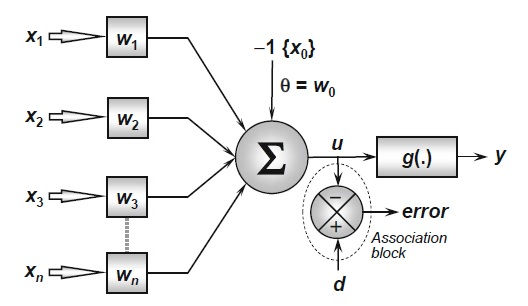
\includegraphics[width=\columnwidth]{ANN.jpg}
      \caption{Red Neuronal Artificial B\'asica}
      \label{fig:fig1}
    \end{figure}

    Donde $\Sigma$ es la representación matemática de la neurona.,  $x_1$, $x_2$,  \dots  ,$x_n$ son las variables de entrada a la red.  $w_1$,$w_2$,  \dots , $w_n$ son los pesos con los cuales se van a podnerar las entradas, es decir multiplicar cuando la información entra en la neurona. Posterior a multiplicar el peso por la entrada correspondiente,  se suman todos esos valores $w_1$$x_1$ + $w_2$$x_2$ + $w_3$$x_3$.

    Al revisar esta formula, se puede observar que se parece a la operación de una regresión la cual es:  $y$ = $w_0$ + $w_i$$x_i$,  de esta forma, internamente la neurona realiza una regresión lineal. En su contraparte, el parámetro que permite a la neurona trazar una recta cruzando el eje $y$ en el plano cartesiano (eje de las ordenadas), a ello se conoce como sesgo (del inglés $bias$),  este valor se agrega a la conexión, el cual usualmente se le da un valor de 1.
    Agregando este nuevo valor a la fórmula, queda de la siguiente manera: $ y = \Sigma w_i x_i + w_0 b$,  donde \textit{b} es el sesgo.

    Un inconveniente del uso de una sola neurona para experimentos es que solo va a resolver ejercicios parecidos a la puerta lógica AND u OR.
    
    Existen problemáticas de solo usar una sola neurona e.g problemas de tipo compuerta XOR.

    Para solucionarlo se usan dos o más neuronas, además de la función de activación, que es la que permite pasar la informaicón de una neurona a otra, en un rango especificado, y la cual se describirá en la siguiente sección.

    \subsection{Función de Activación}

      Dicho método se utiliza cuando el modelo de RNA contiene dos o más neuronas.
      Esta función lo que provoca es dar al modelo una salida no lineal, para eso la segunda fórmula presentada es distorcionada para quedar de la siguiente manera: $f( w_1x_1 + w_2x_2 + w_3x_3 + b_0)$ para el caso de 3 entradas.
      
      Al hablar de funciones de activación se deben de comentar las más comunes, como lo es la función escalonada.

      Tenemos la función escalonada, la cual se representa con la siguiente formula: 
      \[f(x) = \left\{ \begin{array}{lr} 0 & : x < 0\\ 1 & : x \ge 0 \end{array} \right. \]

      Su representación grafica queda de la siguiente manera:
      \begin{figure}[H]
        \centering
        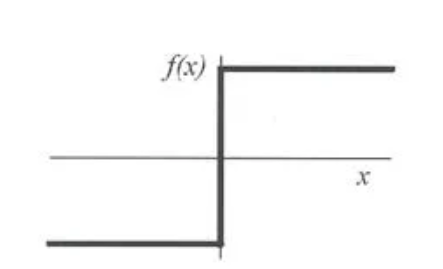
\includegraphics[width=5cm]{staggered.png}
        \caption{Función Escalonada}
        \label{fig:Función Escalonada}
      \end{figure}

      